% ---------------------------------------------------------------------------------------------------------------
% TEMPLATE PARA TRABALHO DE CONCLUSÃO DE CURSO
% Universidade Tecnológica Federal do Paraná - UTFPR
% Customização da classe abnTeX2 (http://www.abntex.net.br/) para as normas da UTFPR
%
% Projeto: http://tcc.tsi.gp.utfpr.edu.br/paginas/modelos-latex-da-utfpr
% Autores: Diego Marczal
% 	       Michael Vornes <https://github.com/mvornes>
%
%----------------------------------------------------------------------------------------------------------------
% Codificação: UTF-8
% LaTeX:  abnTeX2
% ---------------------------------------------------------------------------------------------------------------


% CARREGA CLASSE PERSONALIZADA DA UTFPR--------------------------------------------------------------------------
\documentclass[%twoside,                   % Impressão em frente e verso
    	        oneside,                   % Impressão apenas frente
]{configuracoes/utfpr-abntex2}


% INCLUI ARQUIVOS DE CONFIGURAÇÕES-------------------------------------------------------------------------------
% REFERÊNCIAS------------------------------------------------------------------
\usepackage[%
    alf,
    abnt-emphasize=bf,
    bibjustif,
    recuo=0cm,
    abnt-url-package=url,       % Utiliza o pacote url
    abnt-refinfo=yes,           % Utiliza o estilo bibliográfico abnt-refinfo
    abnt-etal-cite=3,
    abnt-etal-list=3,
    abnt-thesis-year=final
]{abntex2cite}                  % Configura as citações bibliográficas conforme a norma ABNT
% PACOTES----------------------------------------------------------------------

\usepackage{booktabs}                                       % Réguas horizontais em tabelas
\usepackage{color, colortbl}                                % Controle das cores
\usepackage{float}                                          % Necessário para tabelas/figuras em ambiente multi-colunas
\usepackage{graphicx}                                       % Inclusão de gráficos e figuras
\usepackage{icomma}                                         % Uso de vírgulas em expressões matemáticas
\usepackage{indentfirst}                                    % Indenta o primeiro parágrafo de cada seção
\usepackage{microtype}                                      % Melhora a justificação do documento
\usepackage{multirow, array}                                % Permite tabelas com múltiplas linhas e colunas
\usepackage{subeqnarray}                                    % Permite subnumeração de equações
\usepackage{lastpage}                                       % Para encontrar última página do documento
\usepackage{verbatim}                                       % Permite apresentar texto tal como escrito no documento, ainda que sejam comandos Latex

\usepackage{amsfonts, amssymb, amsmath}                     % Fontes e símbolos matemáticos
\usepackage{amsthm}
\usepackage{amscd,latexsym}

%\usepackage{geometry} % just for not getting an overfull box
%\usepackage{bm}

    
    
\usepackage[algoruled, portuguese,linesnumbered]{algorithm2e} % Permite escrever algoritmos em português
\usepackage[bottom]{footmisc}                                 % Mantém as notas de rodapé sempre na mesma posição
\usepackage{ae, aecompl}                                      % Fontes de alta qualidade
\usepackage{latexsym}                                         % Símbolos matemáticos
\usepackage{lscape}                                           % Permite páginas em modo "paisagem"
%\usepackage{picinpar}                                        % Dispor imagens em parágrafos
%\usepackage{scalefnt}                                        % Permite redimensionar tamanho da fonte
%\usepackage{subfig}                                          % Posicionamento de figuras
%\usepackage{upgreek}                                         % Fonte letras gregas
\usepackage[font={footnotesize,bf},center,singlelinecheck=false,tableposition=bottom]{caption}
\usepackage{tabularx}

\usepackage[utf8]{inputenc}                                 % Codificação do documento
\usepackage{fontspec}
%\usepackage[T1]{fontenc}
%\usepackage[scaled]{helvet}                                % Usa a fonte Helvetica
%\usepackage{times}                                         % Usa a fonte Times
%\usepackage{palatino}                                      % Usa a fonte Palatino
%\usepackage{lmodern}                                       % Usa a fonte Latin Modern
%\usepackage{accanthis}
\setmainfont{Times New Roman}[SizeFeatures={Size=12}]
    
\newfontface \helveft{helvetica-bold.otf}
\renewcommand{\captionfont}{\fontsize{8.5}{6}\selectfont{}\helveft}
\renewcommand{\captionlabelfont}{\fontsize{8.5}{6}\selectfont{}\helveft}
    
%\usepackage{indentfirst}

    
%\renewcommand{\familydefault}{\sfdefault}
%\setmainfont{Accanthis ADF Std No3}
%\setromanfont{Accanthis ADF Std No3}
%\setsansfont{Accanthis ADF Std No3}
%\setmonofont{Accanthis ADF Std No3}
    
%% Times New Roman
%\setromanfont[
%BoldFont=timesbd.ttf,
%ItalicFont=timesi.ttf,
%BoldItalicFont=timesbi.ttf,
%]{times.ttf}
%% Arial
%\setsansfont[
%BoldFont=arialbd.ttf,
%ItalicFont=ariali.ttf,
%BoldItalicFont=arialbi.ttf
%]{arial.ttf}
%% Courier New
%\setmonofont[Scale=0.90,
%BoldFont=courbd.ttf,
%ItalicFont=couri.ttf,
%BoldItalicFont=courbi.ttf,
%Color={0019D4}
%]{cour.ttf}



\newtheorem{theorem}{Teorema}
%\newtheorem{acknowledgement}[theorem]{Acknowledgement}
%\newtheorem{algorithm}[theorem]{Afirmação}
%\newtheorem{axiom}{Axioma}
%\newtheorem{case}[theorem]{Caso}
%\newtheorem{claim}[theorem]{Claim}
%\newtheorem{conclusion}[theorem]{Conclusion}
%\newtheorem{condition}[theorem]{Condition}
%\newtheorem{conjecture}[theorem]{Conjectura}
%\newtheorem{corollary}{Corolário}
%\newtheorem{criterion}[theorem]{Criterion}
\newtheorem{definition}{Definição}
%\newtheorem{example}{Exemplo}
%\newtheorem{exercise}{Exercício}
%\newtheorem{lemma}{Lema}
%\newtheorem{notation}{Notação}
%\newtheorem{problem}[theorem]{Problem}
%\newtheorem{proposition}{Proposição}
%\newtheorem{remark}{Observação}
%\newtheorem{solution}[theorem]{Solução}
%\newtheorem{summary}[theorem]{Summary}
%\newenvironment{proof}[1][\textbf{Demonstração:}\hspace{0.2cm}]{\textit{#1}}{\begin{flushright}\itshape{QED.}\end{flushright}}

\usepackage[short,nocomma]{optidef}
\usepackage{blindtext}
\usepackage{pgfplots}
\pgfplotsset{compat=1.9}

\usepackage{hyperref}
\usepackage{tocloft}
\usepackage{etoolbox}

\usepackage{pdfpages}
%\usepackage{xparse}
% load showframe just to show where the box borders are
%\usepackage{showframe}

%\newsavebox{\fminipagebox}
%\NewDocumentEnvironment{fminipage}{m O{\fboxsep}}
% {\par\kern#2\noindent\begin{lrbox}{\fminipagebox}
%  \begin{minipage}{\dimexpr#1-2\fboxsep-2\fboxrule}\ignorespaces}
% {\end{minipage}\end{lrbox}%
%  \fbox{\usebox{\fminipagebox}}%
%  \par\kern#2 }
\include{configuracoes/configuracoes-pdf}


% INCLUI ARQUIVOS DO TRABALHO DE CONCLUSÃO DE CURSO (PRÉ-TEXTUAIS, TEXTUAIS, PÓS-TEXTUAIS)-----------------------

% INSERE CAPA E FOLHA DE ROSTO
% CAPA---------------------------------------------------------------------------------------------------

% ORIENTAÇÕES GERAIS-------------------------------------------------------------------------------------
% Caso algum dos campos não se aplique ao seu trabalho, como por exemplo,
% se não houve coorientador, apenas deixe vazio.
% Exemplos:
% \coorientador{}
% \departamento{}

% DADOS DO TRABALHO--------------------------------------------------------------------------------------
\titulo{Uma análise qualitativa do Sequential Cutting Plane \\ - \\
  da origem às influências modernas}
\titleabstract{Title in English}
\autor{Matheus Machado Vieira}
\autorcitacao{SOBRENOME, Nome} % Sobrenome em maiúsculo
\local{Garanhuns}
\data{2021}

% NATUREZA DO TRABALHO-----------------------------------------------------------------------------------
% Opções:
% - Projeto de Trabalho de Conclusão de Curso de graduação
% - Monografia de Trabalho de Conclusão de Curso (se for Graduação)
% - Dissertação (se for Mestrado)
% - Tese (se for Doutorado)
% - Projeto de Qualificação (se for Mestrado ou Doutorado)
\projeto{}

% TÍTULO ACADÊMICO---------------------------------------------------------------------------------------
% Opções:
% - Bacharel ou Tecnólogo (Se a natureza for Trabalho de Conclusão de Curso)
% - Mestre (Se a natureza for Dissertação)
% - Doutor (Se a natureza for Tese)
% - Mestre ou Doutor (Se a natureza for Projeto de Qualificação)
\tituloAcademico{Bacharel em Ciência da Computação}

% ÁREA DE CONCENTRAÇÃO E LINHA DE PESQUISA---------------------------------------------------------------
% Se a natureza for Trabalho de Conclusão de Curso, deixe ambos os campos vazios
% Se for programa de Pós-graduação, indique a área de concentração e a linha de pesquisa
\areaconcentracao{}
\linhapesquisa{}

% DADOS DA INSTITUIÇÃO-----------------------------------------------------------------------------------
% Se a natureza for Trabalho de Conclusão de Curso, coloque o nome do curso de graduação em "programa"
% Formato para o logo da Instituição: \logoinstituicao{<escala>}{<caminho/nome do arquivo>}
\instituicao{Universidade Federal do Agreste de Pernambuco}
\departamento{} % Deixa em branco caso não exista departamento
\programa{Bacharelado em Ciência da Computação}
\logoinstituicao{0.2}{dados/figuras/logo-instituicao.png}

% DADOS DOS ORIENTADORES---------------------------------------------------------------------------------
\orientador{Gersonilo Oliveira da Silva}
%\orientador[Orientadora:]{Nome da orientadora}
\instOrientador{Universidade Federal do Agreste de Pernambuco}

\coorientador{Rodrigo?????????}
%\coorientador[Coorientadora:]{Nome da coorientadora}
\instCoorientador{Universidade Federal do Agreste de Pernambuco}

% Quando existir mais de um coorientador-----------------------------------------------------------------
% \coorientador[Coorientadores:]{Prof. Me. XXXXXX \newline
% Universidade Tecnológica Federal do Paraná - Câmpus Guarapuava \newline
% \newline Prof. Dr. XXXXX. \newline Universidade Tecnológica
% Federal do Paraná - Câmpus Guarapuava}

% FOLHA DE ROSTO--------------------------------------------------------------------------------------------------------

% TRABALHO DE CONCLUSÃO DE CURSO
\preambulo{Monografia de Trabalho de Conclusão de Curso de
graduação, submetido à Universidade Federal do Agreste de
Pernambuco, como requisito parcial para obtenção do grau
de Bacharel em Ciência da Computação, sob orientação do
professor Dr° Gersonilo Oliveira da Silva.}

% DISSERTAÇÃO DE MESTRADO
% \preambulo{...}

% TESE DE DOUTORADO
% \preambulo{...}

% PROJETO DE QUALIFICAÇÃO DE MESTRADO OU DOUTORADO
%\preambulo{...}


\begin{document}

\pretextual
\imprimircapa                                               	 % Comando para imprimir Capa
\imprimirfolhaderosto{}                                     	 % Comando para imprimir Folha de rosto
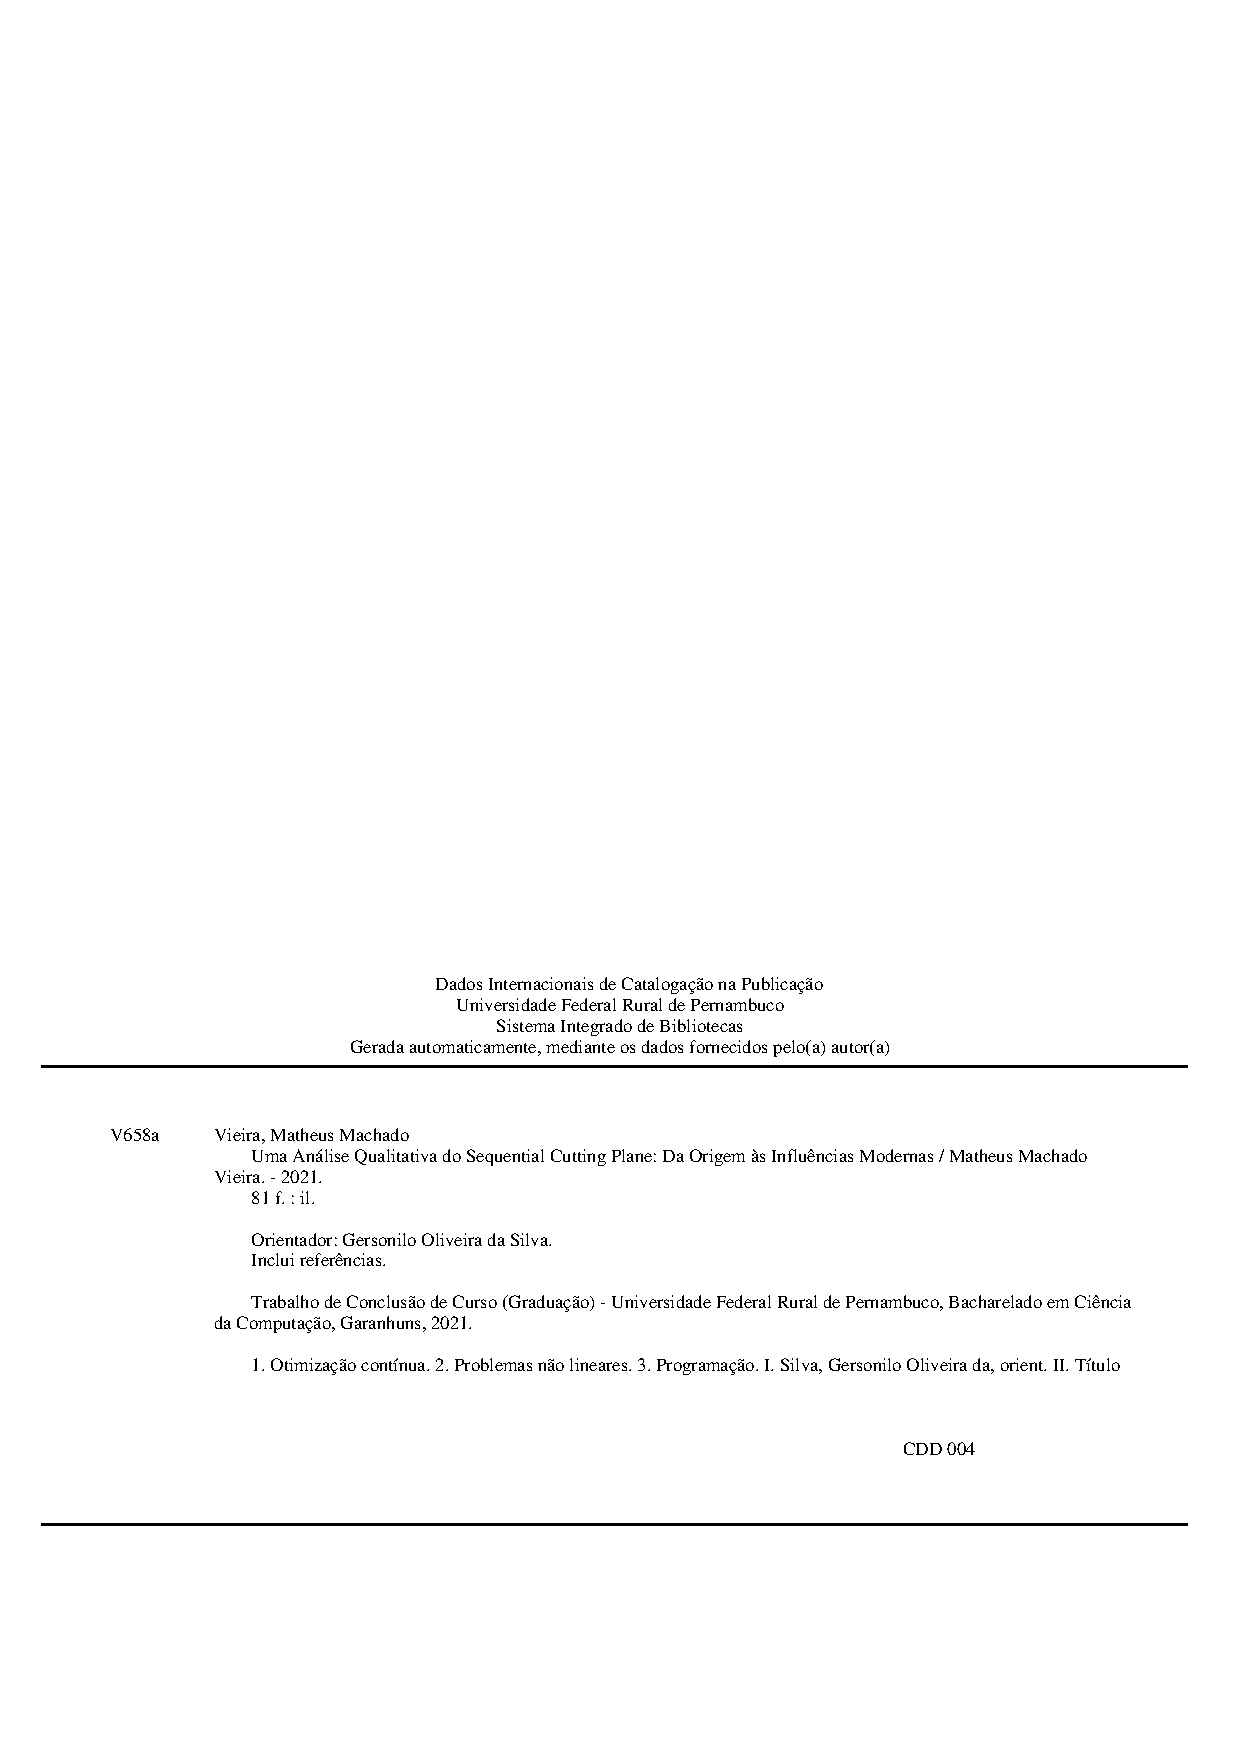
\includepdf[pages=1]{ficha_catalografica}
\imprimirfolhadeaprovacao{}                                  	 % Comando para imprimir Folha de aprovação
% INSERE ELEMENTOS PRÉ-TEXTUAIS
%\include{estrutura/pre-textuais/dedicatoria}          			   % Dedicatória
%% AGRADECIMENTOS---------------------------------------------------------------

\begin{agradecimentos}[\larger Agradecimentos]

Edite e coloque aqui os agradecimentos às pessoas e/ou instituições que contribuíram para a realização do trabalho.

É obrigatório o agradecimento às instituições de fomento à pesquisa que financiaram total ou parcialmente o trabalho, inclusive no que diz respeito à concessão de bolsas.

\end{agradecimentos}
        			   % Agradecimentos
%\include{estrutura/pre-textuais/epigrafe}              			   % Epígrafe
% RESUMO--------------------------------------------------------------------------------

\begin{resumo}[\larger Resumo]
%\begin{SingleSpacing}

% Não altere esta seção do texto--------------------------------------------------------
%\imprimirautorcitacao. \imprimirtitulo. \imprimirdata. \pageref {LastPage} f. \imprimirprojeto\ – \imprimirprograma, \imprimirinstituicao. \imprimirlocal, \imprimirdata.\\
%---------------------------------------------------------------------------------------

O Resumo é um elemento obrigatório em tese, dissertação, monografia e TCC, constituído de uma seqüência de frases concisas e objetivas, fornecendo uma visão rápida e clara do conteúdo do estudo. O texto deverá conter no máximo 500 palavras e ser antecedido
pela referência do estudo. Também, não deve conter citações. O resumo deve ser redigido em parágrafo único, espaçamento simples e seguido das palavras representativas do conteúdo do estudo, isto é, palavras-chave, em número de três a cinco, separadas entre si por ponto e finalizadas também por ponto. Usar o verbo na terceira pessoa do singular, com linguagem impessoal, bem como fazer uso, preferencialmente, da voz ativa. Texto contendo um único parágrafo.\\

\textbf{Palavras-chave}: Palavra. Segunda Palavra. Outra palavra.

%\end{SingleSpacing}
\end{resumo}

% OBSERVAÇÕES---------------------------------------------------------------------------
% Altere o texto inserindo o Resumo do seu trabalho.
% Escolha de 3 a 5 palavras ou termos que descrevam bem o seu trabalho
%
% Adequação das palavras chaves, a biblioteca solicitou que todos adequem as
% palavras chaves de acordo com as cadastras no sistema de disponibilização de
% trabalhos da biblioteca.

% Segue as instruções: A busca por palavra chave é feita da seguinte forma:
% Acessar o site da biblioteca nacional: http://acervo.bn.br/sophia_web/; Clicar
% em autoridades; Em busca por autoridade selecionar "termo tópico"; Selecionar
% "iniciar com"; Digitar a palavra que se quer verificar se está cadastrada (ex:
% sistemas) e após buscar; Note que no ex. "sistemas" apareceram várias opções
% (Sistemas auto-organizáveis, Sistemas CAD/CAM, Sistemas de avaliação de risco
% de crédito), o número 16 corresponde à "sistemas de computação". Clicando nesse
% termo aparecem 3 abas, as quais se pode verificar se realmente é o termo
% procurado; Na aba MARC Tag usamos o número 150 para a palavra-chave em
% português e o número 750 para a palavra-chave em inglês.
             			     % Resumo em Português
% ABSTRACT--------------------------------------------------------------------------------

\begin{resumo}[\larger Abstract]
%\begin{SingleSpacing}

% Não altere esta seção do texto--------------------------------------------------------
%\imprimirautorcitacao. \imprimirtitleabstract. \imprimirdata. \pageref {LastPage} f. \imprimirprojeto\ – \imprimirprograma, \imprimirinstituicao. \imprimirlocal, \imprimirdata.\\
%---------------------------------------------------------------------------------------

Elemento obrigatório em tese, dissertação, monografia e TCC. É a versão do resumo em português para o idioma de divulgação internacional. Deve ser antecedido pela referência do estudo. Deve aparecer em folha distinta do resumo em língua portuguesa e seguido das palavras representativas do conteúdo do estudo, isto é, das palavras-chave. Sugere-se a elaboração do resumo (Abstract) e das palavras-chave (Keywords) em inglês; para resumos em outras línguas, que não o inglês, consultar o departamento / curso de origem.\\

\textbf{Keywords}: Word. Second Word. Another word.

%\end{SingleSpacing}
\end{resumo}

% OBSERVAÇÕES---------------------------------------------------------------------------
% Altere o texto inserindo o Abstract do seu trabalho.
% Escolha de 3 a 5 palavras ou termos que descrevam bem o seu trabalho 
             		                % Resumo em Inglês
\include{estrutura/pre-textuais/listas/listas-ilustracoes/lista-figuras}  % Lista de Figuras
%\include{estrutura/pre-textuais/listas/listas-ilustracoes/lista-quadros}  % Lista de Quadros
\include{estrutura/pre-textuais/listas/lista-tabelas}         		        % Lista de Tabelas
% LISTA DE ABREVIATURAS E SIGLAS----------------------------------------------------------

\begin{siglas}
\item[ARC] Atualização da Região de Confiança
\item[BFGS] Broyden–Fletcher–Goldfarb–Shanno
%\item[CAPES] Coordenação de Aperfeiçoamento de Pessoal de Nível Superior
\item[CPU] Central Processing Unit
\item [DFP] Davidon–Fletcher–Powell
\item[EMFCQ] Extented Mangasarian-Fromovitz Constraint Qualification
\item[KKT] Karush-Kuhn-Tucker
\item[KKTE] KKT Estacionário
\item[MINLP] Mixed Integer Nonlinear Programming
\item[SCP] Sequential Cutting Plane, Sequential Convex Programming
\item[SPL] Sequência de Problemas Lineares
\item[SQP] Sequential Quadratic Programming
%\item[UFAPE] Universidade Federal do Agreste de Pernambuco
\item[VFM] Verificação da Função de Mérito
\end{siglas}

% OBSERVAÇÕES-----------------------------------------------------------------------------
% Altere a lista acima para definir os acrônimos e siglas utilizados neste trabalho
          		        % Lista de Abreviaturas e Siglas
%\include{estrutura/pre-textuais/listas/lista-simbolos}        		        % Lista de Símbolos
\include{estrutura/pre-textuais/listas/listas-diversas/lista-algoritmos}  % Lista de Algoritmos
% SUMÁRIO----------------------------------------------------------------------
\setlength\cftchapternumwidth{2em}

\renewcommand{\contentsname}{SUMÁRIO}

%\makeatletter
%\settocpreprocessor{chapter}{%
%    \let\tempf@rtoc\f@rtoc% 
%    \def\f@rtoc{%
%      \texorpdfstring{\MakeUppercase{%
%        \tempf@rtoc}%
%      }{\tempf@rtoc}%
%    }%
%}
%\makeatother
%   
%\renewcommand{\cftsectionfont}{\MakeUppercase}
%\renewcommand{\cftsubsectionfont}{\bfseries}
    
\pdfbookmark[0]{\contentsname}{toc}
\tableofcontents*
\cleardoublepage

% OBSERVAÇÕES-------------------------------------------------------------------
% Este arquivo não precisa ser alterado, pois o sumário é gerado automaticamente.
               			              % Sumário

\textual
% INSERE ELEMENTOS TEXTUAIS
% INTRODUÇÃO-------------------------------------------------------------------

\chapter{\larger Introdução}
\label{chap:introducao}

Edite e coloque aqui o seu texto de introdução.

A Introdução é a parte inicial do texto, na qual devem constar o tema e a delimitação do assunto tratado, objetivos da pesquisa e outros elementos necessários para situar o tema do trabalho, tais como: justificativa, procedimentos metodológicos (classificação inicial), embasamento teórico (principais bases sintetizadas) e estrutura do trabalho, tratados de forma sucinta. Recursos utilizados e cronograma são incluídos quando necessário. Salienta-se que os procedimentos metodológicos e o embasamento teórico são tratados, posteriormente, em capítulos próprios e com a profundidade necessária ao trabalho de pesquisa.

\section{LEIA ESTA SEÇÃO ANTES DE COMEÇAR}
\label{sec:antesleiame}

Este documento é um \emph{template} \LaTeX{} que foi concebido, primariamente, para ser utilizado na elaboração de Trabalho de Conclusão de Curs em conformidade com as normas da Universidade Tecnológica Federal do Paraná.

Para a produção deste \emph{template} foi necessário adaptar o arquivo {\ttfamily abntex2.cls}. Assim, foi produzido o arquivo {\ttfamily utfpr-abntex2.cls} que define o \verb|documentclass| específico para a UTFPR.

Antes de começar a escrever o seu trabalho acadêmico utilizando este \emph{template}, é importante saber que há dois arquivos que você precisará editar para que a capa e a folha de rosto de seu trabalho sejam geradas automaticamente.
São eles os arquivos {\ttfamily capa.tex} e {\ttfamily folha-rosto.tex}, ambos no diretório  {\ttfamily /elementos-pre-textuais}.
No arquivo {\ttfamily capa.tex} deverá ser informado nome do autor, título do trabalho, natureza do trabalho, nome do orientador e outras informações necessárias.
No arquivo {\ttfamily folha-rosto.tex}, que contém o texto padrão estabelecendo que este documento é um requisito parcial para a obtenção do título pretendido, será necessário apenas comentar as linhas que não se aplicam ao tipo de trabalho acadêmico.

A compilação para gerar um arquivo no formato pdf, incluindo corretamente as referências bibliográficas, deve ser realizada utilizando o comando \verb|makefile|, disponível na mesma pasta onde está o arquivo principal \verb|utfpr-tcc.tex|. Caso seja alterado o nome do arquivo \verb|utfpr-tcc.tex|, deverá ser alterado no arquivo \verb|makefile| também.

\section{ORGANIZAÇÃO DO TRABALHO}
\label{sec:organizacaoTrabalho}

Normalmente ao final da introdução é apresentada, em um ou dois parágrafos curtos, a organização do restante do trabalho acadêmico.
Deve-se dizer o quê será apresentado em cada um dos demais capítulos.
                		           % Introdução
% REVISÃO DE LITERATURA--------------------------------------------------------

\chapter{\larger Revisão Literária}
\label{chap:fundamentacaoTeorica}

É uma boa prática iniciar cada novo capítulo com um breve texto introdutório (tipicamente, dois ou três parágrafos) que deve deixar claro o quê será discutido no capítulo, bem como a organização do capítulo.
Também servirá ao propósito de "amarrar"{} o conteúdo deste capítulo com o conteúdo do capítulo imediatamente anterior.

\section{A programação sob o viés matemático}
Esboço de um resumo dos dois primeiros capítulos do livro de otimização, o que vai justificar muita coisa na verdade temos que ver depois v
\subsection{Otimizando à uma variável}
\subsection{Otimizando à mais de uma variável}

%subscheqchion

\section{As primeiras três décadas da programação}
(1930-1960)
Dantzing, M, até -SQP.
\section{Programação não linear - O surgimento}
\section{Os pilares arquitetônicos do SCP}
\section{O modernismo sob o ponto de vista da programação (Uma ideia do o quê que a gente tem de moderno)}
   % Revisão de Literatura
% METODOLOGIA------------------------------------------------------------------

\chapter{\larger Percurso Metodológico}
\label{chap:metodologia}
Cada capítulo deve conter uma pequena introdução (tipicamente, um ou dois parágrafos) que deve deixar claro o objetivo e o que será discutido no capítulo, bem como a organização do capítulo.

\section{DELINEAMENTO DA PESQUISA}
\label{sec:titSecDelPesq}

Inserir seu texto aqui...

\section{COLETA E TRATAMENTO DE DADOS}
\label{sec:titSecColDad}

Inserir seu texto aqui...
             % Metodologia
% RESULTADOS-------------------------------------------------------------------

\chapter{\larger Análise e discussão dos resultados}


TODO: explicar que a ideia dos algoritmos são minhas
TODO: Cada capítulo deve conter uma pequena introdução (tipicamente, um ou dois parágrafos) que deve deixar claro o objetivo e o que será discutido no capítulo, bem como a organização do capítulo.


\section{O modernismo sob o ponto de vista da programação}
Ao observarmos o percusso histórico dos métodos de otimização, podemos ir tão atrás no tempo
quanto a matemática é usada, mas para que possamos considerar passagens de eras é necessário
buscar acontecimentos com uma certa relevância, e que tais acontecimentos estejam relacionados
a contextos de relevância na época.

Um grande acontecimento que podemos tomar como algo que marque a passagem de uma era para
outra é o desenvolvimento do cálculo por Newton (sabe-se que existem outros, mas Newton é
o mais creditado). Ao observarmos o que seria um processo de otimização matemática prévio
ao cálculo, vemos que parece ser algo de certa forma não tão eficiente ou prático. Mesmo
considerando um problema simples, tomando que sua interpretação por meio de gráficos bastaria
para uma resolução do problema, não seria algo tão trivial como percebemos hoje, uma vez
que até a própria estruturação de problemas gráficos era algo recente no momento de Newton,
já que a estruturação de coordenadas do plano acabava de ser feita por Descartes.

Logo após o desenvolvimento do cálculo, toda uma nova forma de se considerar problemas
que já existiam ou ainda derivar novos problemas foi conhecida. Nomes como Bernoulli, Euler,
Cauchy (\ref{secao_historia}) Weierstrass (\ref{Teorema_de_Weierstrass}) comprovam a rápida
aceitação das ideias de cálculo e análise matemática, como também formam bases sólidas para
o que temos sobre otimização atualmente. Métodos já tinham sido propostos, bem como algumas
de suas propriedades, como o próprio método de Newton (em colaboração com Raphson), ou ainda
a primeira aparição do método do gradiente descendente, por Cauchy.

Desde essa época, o estudo da otimização foi tomando ramos e se especializando cada vez mais.
As especializações normalmente surgem de acordo com modelos de problemas reais que deseja-se
otimizar, por isso hoje somos capazes de encontrar toda uma vasta bibliografia a respeito de
otimização de problemas lineares, não lineares, considerando variáveis inteiras, variáveis
reais, ou ambas.

Ao considerarmos os interesses de cada época em aprimorar o conhecimento matemático, podemos
perceber acontecimentos que estão relacionados a esses interesses. Ao tomarmos como um ponto
de partida o movimento iluminista no século XVIII, vemos e sabemos a relação com os estudos
de Newton e os mesmos de sua época, e também compreendemos que o ideal iluminista contribuiu
bastante para a disseminação desses estudos. Um segundo acontecimento que podemos levar em
consideração é a revolução industrial. Conceitos físicos de máquinas pensadas durante a
revolução industrial são construídos sobre a nova fundação do cálculo, permitindo, dentre
outras coisas, melhor eficiência das máquinas. Podemos dizer que um dos pontos altos desse
período, mesmo que tardio, é o trabalho de Maxwell sobre a termodinâmica, o qual, de forma
geral, é baseado em conceitos de estabilidade de sistemas.


O movimento de industrialização sempre crescente começou a demonstrar seus pontos fracos,
principalmente em relação às eficiências das indústrias, ainda no começo do século XX,
quando as demandas cresceram, logísticas sobre recursos de produção foram dificultadas,
e tensões internacionais estavam se formando. Passada a Primeira Guerra Mundial, diversos
países se encontram com recursos escassos e buscando mais atenção no gerenciamento desses
recursos. Essa atenção nos leva à dois nomes que desenvolveram, de certa forma, as mesmas
ferramentas para as mesmas finalidades, Kantorovich(\ref{sec_kantorovich}) e Dantzig
(\ref{sec_dantzig}), ambos buscando otimizar o processo de alocação de pessoas, recursos,
ou algo em relação com o potencial de produção. Mesmo havendo um interesse maior em
otimização linear nesse período, outras áreas da otimização vinham sendo desenvolvidas
também, um exemplo disso são as condições KKT (\ref{sec_kkt}).

Agora após a Segunda Guerra Mundial, os computadores digitais começam a ganhar mais espaço.
Na década de 50, como uma das primeiras linguagens de programação, temos o Fortran, do
inglês Formula Translation, como sendo uma linguagem pensada para os cálculos matemáticos
precisos e custosos de se fazer manualmente. Junto a isso, o recém desenvolvimento da otimização
linear e as novas bases formadas para outras áreas da otimização expandiu o interesse que
se tinha na época.

Quando chegamos na década de 60, encontramos os nomes e acontecimentos já citados na seção
\ref{secao_historia}, os quais agora podem ser compreendidos como em uma era moderna. E
seguindo daí, não é mais tão claro um acontecimento com influência na otimização para
podermos separar uma nova era.

Olhando agora para o lado dos computadores, enquanto a otimização já estava em seu
período moderno, os computadores estavam apenas começando, sendo usados mainframes
para cálculos já computacionalmente desenvolvidos, o que acabava restringindo o
acesso ao estudo nesse meio, mesmo considerando o interesse crescente no assunto.
Considerando os avanços rápidos, Fortran nunca deixou de ser usada e atualizada,
um exemplo é que ainda hoje diversas bibliotecas matemáticas em fortran são usadas.
Avanços, como invenção e difusão de linguagens estruturadas (C e Ada) contribuíram
na difusão e acessibilidade dos estudos sobre otimização, tanto que o DONLP2
(\ref{sec_dosnlp2}) que foi escrito em C, e Ada é uma linguagem usada até hoje
como linguagem para sistemas críticos, como sistemas operacionais da aviação.

Agora considerando como um todo a análise histórica apresentada no capítulo
\ref{chap:fundamentacaoTeorica}, o SCP se encaixa em um contexto com um ideal
semelhante ao renascentismo. É dito na apresentação do SCP que um de seus objetivos
é recuperar o interesse no uso de técnicas de resolução de subproblemas lineares
que haviam sido deixados de lado em favor dos métodos quadráticos. Considerando
os resultados obtidos pelos autores do SCP, foi mostrado por eles que houve
um avanço para outras técnicas de otimização sem antes esgotar as possibilidades
do que os problemas lineares tinham a oferecer. Podemos ver isso ao considerar
que as técnicas empregadas no SCP já existiam, ou pelo menos tinham suas bases
firmes, no momento que os métodos quadráticos ganharam sua fama. Dito isso, podemos
colocar o SCP como sendo um método pós-moderno/renascentista, também considerando
a década de sua concepção, de 2000 à 2010.







\section{Introdução ao SCP}
O Sequencial Cutting Plane (SCP) \cite{Still2010} pode ser visto como uma demonstração da
capacidade das técnicas de otimização por problemas lineares que, como já dito, haviam
sido deixadas de lado. O método apresentado por Claus Still e Tapio Westerlund em 2010
pode ser visto como a conclusão do estudo deles sobre abordagens de subproblemas lineares
em problemas não lineares. Um estudo de pelo menos 5 anos, com o primeiro artigo sendo
uma apresentação do método em um estagio inicial aplicado a problemas de otimização
não linear inteira mista (MINLP) \cite{Still_2005}.

O método foi primariamente aplicado em problemas MINLP como parte de um algoritmo,
demonstrando melhor performance em problemas MINLP convexos. Outra possibilidade de
aplicação é o uso para resolução de problemas não lineares de grande escala, de grande
dimensionalidade, visto a problemática enfrentada por métodos quadráticos para tais
problemas.



\subsection{Aplicação SCP em MINLP}
Uma das aplicações do SCP foi como parte de um otimizador de outra classe de problemas, na
otimização não linear inteira mista (MINLP). Existem problemas que buscam o ótimo usando
variáveis tanto discretas como continuas, com relações entre elas que são não lineares e
que também contém funções não convexas. Tudo isso dificulta muito a computação da solução.
Otimizadores capazes de resolverem esses tipos de problemas são ditos como os mais flexíveis,
já que seu escopo é tão abrangente. Isso o torna o centro das atenções por pesquisadores de
todas as áreas.

Problemas MINLP, na sua forma mais abstrata se dão da seguinte forma:

\vspace{-15pt}
\begin{mini!}
{x}{ f(x) \label{minlp_obj}}{\label{prob_minlp}}{}
\addConstraint{x}{\in \mathcal{F} \subseteq \mathbb{R}^n}{\label{r1_minlp}}
\end{mini!}
onde o conjunto \( \mathcal{F} \) pode ser tanto não linear quanto discreto, e \( f: \mathbb{R}^n \mapsto \mathbb{R}\) .
As diferentes escolhas
de \(f\) e \(\mathcal{F}\) levam as diferentes subclasses de MINLP, das quais temos algumas
denominações mais comuns, como:

\begin{itemize}
\item Otimização Convexa, onde \( \mathcal{F} \) é convexo, e o ótimo é inteiro;
\item Otimização Disjuntiva, onde algumas variáveis são continuas e outras são booleanas;
\item Otimização Não Linear, onde restrições não lineares constroem \(\mathcal{F}\) e/ou \(f\) é não linear. Normalmente usados métodos SQP;
\item Otimização por meio de grafos de expressões;
\item Otimização por meio de subespaços convexos e/ou linearizações de \(\mathcal{F}\).
\end{itemize}

Podemos encontrar que as formas mais gerais de MINLP são incomputáveis, visto que pode não existir
informações ou ferramentas para serem usadas na resolução do problema. Para problemas MINLP convexos,
e com restrições de desigualdades, a resolução de subproblemas lineares oferecem limites inferiores para
o ótimo, o que para o SCP, saber desses limites ajuda em questões de eficiência. Segundo os autores do
SCP, ao ser usado para problemas MINLP, foram encontradas soluções melhores em apenas um minuto do que
usando outros métodos que encontraram boas soluções em 12 horas.

A resolução de problemas MINLP convexos é importante no contexto global de problemas MINLP, já
que a maioria dos problemas são resolvidos por uma sequência de problemas que foram convertidos em
problemas convexos. Experiências numéricas mostram que o SCP pode ser aplicado para problemas MINLP
não convexos como solucionador de subproblemas. A convergência ao ponto estacionário, quando aplicado
a estes tipos de problemas, aparenta ser rápida o suficiente mesmo que o estado do algoritmo esteja
longe do ponto estacionário.



\section{Análise Qualitativa do algoritmo - SCP}
%TODO: --
%\begin{enumerate}
%\item copiar o pseudo codigo do scp
%\item analisar minuciosamente cada etapada do algoritmo
%\item ENTREGAR 07/06/2021 AS 16 O CAPTULO 4 TODO E INTEIRO
%\end{enumerate}


%\subsection{Problema resolvido pelo SCP}
O SCP resolve problemas no seguinte formato:

\vspace{-15pt}
\begin{mini!}
{x}{ f(x) \label{scp_obj}}{\label{prob_scp}}{}
\addConstraint{g_j(x)}{\leq 0, \quad}{j = 1, ..., m_i \label{r1_scp}}
\addConstraint{h_r(x)}{= 0, \quad}{r = 1, ..., m_e \label{r2_scp}}
\end{mini!}

Onde todas as funções devem ser continuamente diferenciáveis em \(\mathbb{R}^n\) assim como
devem ser funções \( \mathbb{R}^n \mapsto \mathbb{R} \). Nenhuma função é considerada convexa e isto
pode ser visto como um avanço à forma anterior do método. A única coisa assumida é que alguma das
funções \( g_j(x) \) é linear. Com isso podemos perceber que o SCP é capaz de trabalhar com uma
grande quantidade de problemas, visto que essa forma de problema pode ser modelada de aplicações
em diversas áreas.

Outra coisa que é assumida, é que as qualificações de restrições de Mangasarian-Fromovitz estendidas (EMFCQ)
\cite{di1994exact} são válidas para qualquer \( x \in \mathbb{R}^n \), como visto na seção \ref{sec_emfcq}.
%\cite{di1994exact} são válidas para qualquer \( x \in \mathbb{R}^n \) de forma que, \( \nabla h_r(x) \), para
%\(r = 1, ..., m_e\), sejam linearmente independentes e que:

%\vspace{-15pt}
%\begin{flalign}
%  & \exists z \in \mathbb{R}^n \\
%  & \nabla g_j(x)^T z < 0, j \in (J_+(x) \cup J_0(x)) \\
%  & \nabla h_r(x)^T z = 0, r = 1, ..., m_e
%\end{flalign}
%onde \( J_+(x) := \{j | g_j(x) > 0\} \) é o conjunto de restrições violadas e
%\( J_0(x) := \{j | g_j(x) = 0\} \) é o conjunto de restrições que estão na fronteira
%da região limitada por elas.
%
Estas qualificações garantem que, para qualquer ponto não viável, exista uma
direção de descida em direção a uma região viável. Existe também uma relação entre as EMFCQ
e funções de penalidade exatas.


\subsection{O Algoritmo}
O algoritmo é iterativo, assim como no clássico método de Newton se é gerada
uma sequência de pontos convergentes para um ponto ótimo.
Cada uma de suas iterações consiste em um conjunto de subiterações de
resolução de problemas lineares. A cada problema linear resolvido, é obtida
uma direção de descida, e com essa direção, é feita uma busca em linha,
buscando um tamanho ótimo para o passo. Após essas iterações de problemas
lineares, é esperado que um novo ponto capaz de reduzir suficientemente uma
função de mérito, o que garante a convergência.



\begin{algorithm}[H]
  \SetAlgoLined
  \( k \gets 1 \)\;
  \( H_k \gets I \)\;
  \( x_k \gets \) ponto inicial\;
  
  \While{k \(\leq\) Iterações máximas}{
    \((d_k, x_{k+1}, H_{k+1}, \lambda_{k+1}, \mu_{k+1}, est) \gets SPL(x_k, H_k) \) \tcp{Problemas lineares}

    \If{est = true} {
      break \tcp*{Para se foi encontrado um ponto KKT estacionário}
    }

    \(x_{k+1} \gets VFM(d_k, x_k, \lambda_k, \mu_k, x_{k+1}, \lambda_{k+1}, \mu_{k+1})\) \tcp*{Verificação de descida}
    \(ARC(x_k, x_{k+1})\)\tcp*{Atualização das regiões de confiança}
    
    \If{\(KKTE(x_{k+1}, \lambda_{k+1}, \mu_{k+1})\) = true} {
      break \tcp*{Para se foi encontrado um ponto KKT estacionário}
    }
    
    \(k \gets k + 1\)

  }
  \caption{SCP}
\end{algorithm}
\vspace{15pt}


A função \(SPL\) é responsável por resolver a sequência de problemas lineares
buscando direções ótimas de descida enquanto já desloca o ponto atual. A função
\(VFM\) é responsável por fazer a verificação da qualidade do novo ponto encontrado
por \(SPL\), se o ponto satisfizer as condições impostas, ele é mantido, caso contrário
é buscado um que satisfaça por outros meios. A função \(ARC\) verifica o tamanho da região
de confiança para as soluções \(d\) encontradas em \(SPL\). Por fim, \(KKTE\) verifica
se o ponto é um KKT estacionário do problema. Quando o algoritmo para, o ponto
mais recente adicionado à sequência é a solução, \(x_k\) se foi atingido
o número máximo de iterações, ou \(x_{k+1}\) em uma parada por ponto
estacionário.

\subsubsection{Subiterações lineares}

Cada subiteração linear é a resolução de um problema linear fixado no ponto
atual \( x_i \), \(i\) sendo a iteração linear atual. O problema linear que
será resolvido é dado por:


\vspace{-15pt}
\begin{mini!}
{x}{   \nabla f(x_i)^T d + C(\sum_{j=1}^{m_i} t_j^g + \sum_{r=1}^{m_e} t_r^{h^+} + \sum_{r=1}^{m_e} t_r^{h^-}) \label{scpl_obj}}{\label{prob_scpl}}{}
\addConstraint{g_j(x_i) + \nabla g_j(x_i)^T d}{ \leq t_j^g, \quad}{j = 1, ..., m_i \label{r1_scpl}}
\addConstraint{h_r(x_i) + \nabla h_r(x_i)^T d}{= t_r^{h^+} - t_r^{h^-}, \quad}{r=1, ..., m_e \label{r2_scpl}}
\addConstraint{(d_r)^T (H_i d)}{= 0, \quad}{r=1, ..., i-1, i > 1 \label{r3_scpl}}
\addConstraint{d^L \leq d}{\leq d^U}{ \label{r4_scpl}}
\addConstraint{0 \leq t_j^g}{\leq max(g_j(x_i), 0), \quad}{j=1, ..., m_i \label{r5_scpl}}
\addConstraint{0 \leq  t_r^{h^+}}{\leq |h_r(x_i)|, \quad}{r = 1, ..., m_e \label{r6_scpl}}
\addConstraint{0 \leq  t_r^{h^-}}{\leq |h_r(x_i)|, \quad}{r = 1, ..., m_e \label{r7_scpl}}
\end{mini!}
com a solução sendo \( d, t^g, t^{h^+}, t^{h^-} \).

As restrições (\ref{r1_scpl}) e (\ref{r2_scpl}) são versões lineares das restrições originais,
onde a busca por um \(d_i \) que resolva o problema garante que na próxima iteração, o ponto já não
viole restrições. As variáveis \(t^g\), \(t^{h^+}\), \(t^{h^-}\), são relaxamentos das restrições,
o que facilita encontrar um \(d_i\) dentro de (\ref{r4_scpl}).

A restrição (\ref{r3_scpl}) faz com que a direção de descida \( d_i \) seja H-conjugada (\ref{aortogonal}) à todas
as outras direções encontradas anteriormente por outras subiterações lineares desta
interação não linear. \( H_i \) é a matriz hessiana da função Lagrangiana (\ref{fn_lagrangiana}) do problema
original, também avaliada no ponto \( x_i \).

Não é necessária mais que uma iteração de resolução de problema linear para
que o algoritmo venha a convergir, mas ainda assim pode ser feito para melhorar a velocidade
de convergência. Como é necessário que a cada iteração linear a solução
\( d_i \) seja conjugada à todos os outros \(d\)s de iterações lineares anteriores, o
algoritmo busca uma direção de descida que "aponte" mais certeiramente para o ótimo.
Por esse motivo esse método lembra o gradiente conjugado, quando essa restrição é
considerada.

A restrições (\ref{r4_scpl}) nada mais são que um paralelepípedo que limita o espaço de busca de uma
direção descida. Onde \( d^L < \overrightarrow 0 \) e \( d^U > \overrightarrow 0 \).

As linearizações vistas em (\ref{r1_scpl}) e (\ref{r2_scpl}) e o requerimento de ortogonalidade entre
as direções de descida encontradas em respeito à Lagrangiana da função em (\ref{r4_scpl}) são (hiper)planos
que cortam o espaço.

As restrições (\ref{r1_scpl}) são linearizações que geram uma região no espaço que aproxima a região viável
das restrições \( g_j(x), j=1, ..., m_i \). Da mesma forma (\ref{r2_scpl}) são (hiper)planos que aproximam
também a região limitada de \( h_r(x), r=1, ..., m_e \).

Por fim as restrições (\ref{r5_scpl}), (\ref{r6_scpl}) e (\ref{r7_scpl}) controlam o quanto a função objetivo
(\ref{scpl_obj}) é relaxada em relação às restrições que não estão sendo satisfeitas. Quando todas as restrições
são satisfeitas em \(x_i\), vemos que \( t^g \) ,\(t^{h^+}\) e \(t^{h^-} \) são todos nulos.


Para a implementação da função \(SPL\) precisamos inicialmente de uma forma de gerar o problema linear
(\ref{prob_scpl}), que uma vez gerado, deve ser resolvido. O próximo passo a ser tomado é resolver
o problema dual de (\ref{prob_scpl}), uma vez que a solução do problema dual pode ser usada como estimativa
dos multiplicadores de Lagrange. Após isso, já temos a possibilidade de verificar se o ponto atual é um
ponto KKT estacionário (visto a necessidade dos multiplicadores de Lagrange para isso). Caso seja KKT
estacionário já podemos retornar as informações necessárias, do contrário, é feita uma busca em linha
buscando um tamanho para o passo na direção encontrada na solução do problema linear. Essa busca em
linha é feita em uma função Lagrangiana penalizada de acordo com as restrições cumpridas. Uma vez
encontrado o tamanho do passo, o ponto da interação atual pode ser atualizado como no método de gradiente
descendente. Agora, a depender de como foi escolhido, é computada a matriz Hessiana da função Lagrangiana
para a próxima iteração. Por fim, caso algum dos critérios de parada de subiterações lineares forem
satisfeitos, retornamos as informações obtidas até agora, caso contrário, repetimos o processo tomando
o ponto atualizado como o novo ponto de partida.


\vspace{15pt}
\begin{algorithm}[H]
  \SetAlgoLined
  \SetKwFunction{FSPL}{SPL}
  \SetKwProg{Fn}{Function}{:}{}
  \Fn{\FSPL{\(x_k, H_k\)}}{
    \(i \gets 1\)\;
    \(x_i \gets x_k\)\;
    \(H_i \gets H_k\)\;
      
  \While{Condições de parada não satisfeitas}{
    \( (A, b, c) \gets gerar\_problema(x_i, H_i) \)\;
    \(( d_i, t^g_i, t^{h^+}_i, t^{h^-}_i) \gets primal(A, b, c) \)\;
    \((\lambda_i, \mu_i)  \gets dual(A, b, c)\)\;
    
    \If{\(KKTE(x_i, \lambda_i, \mu_i)\) = true} {
      \KwRet \((d_i, x_i, H_i, \lambda_i, \mu_i, true)\)\;
    }

    \(\alpha_i \gets busca\_em\_linha\_lagrangiana\_penalizada(x_i, d_i, \lambda_i, \mu_i)\)\;
    \(x_{i+1} \gets x_i + \alpha_i d_i \)\;
    \(H_{i+1} \gets hessiana(x_i, x_{i+1})\)\;
    \(i \gets i + 1\)\;
  }
  
  \KwRet \((d_i, x_i, H_i, \lambda_i, \mu_i, false)\)\;
  }
  \caption{SPL}
\end{algorithm}
\vspace{15pt}


Para a geração e resolução do problema é necessário compreender o formato dele e ajusta-lo
para a melhor forma possível de resolver. Para isso, vamos considerar o seguinte problema
de minimização linear e seu dual:

\begin{mini!}
{x}{ c^Tx}{\label{prob_linear_pdr}}{}
\addConstraint{Ax}{\geq b}{\label{dr12}}
\end{mini!}

\begin{maxi!}
{y}{ b^Ty}{}{}
\addConstraint{A^Ty}{= c}{\label{dr12}}
\end{maxi!}

Para que possamos resolver (\ref{prob_scpl}) com facilidade pelos métodos convencionais,
temos que transforma-lo na tripla \(A, b, c\) dos problemas acima, e com isso, também
considerar apenas um único vetor solução \(x\). Tomemos \(x\) como sendo
\((d, t^g, t^{h^+}, t^{h^-})\), logo, um vetor do \(\mathbb{R}^{n + m_i + m_e + m_e}\).
Podemos perceber rapidamente o que é o vetor \(c\) a partir de (\ref{scpl_obj}),
que as primeiras entradas são \(\nabla f(x_i)\) e todo o resto é o escalar de
relaxamento \(C\). Para a matriz \(A\) e o vetor \(b\) precisamos primeiro
reescrever as restrições de forma que fique clara as entradas. Podemos reescrever
(\ref{prob_scpl}) da seguinte forma:

\vspace{-15pt}
\begin{mini!}
{x}{   \nabla f(x_i)^T d + \sum_{j=1}^{m_i}Ct_j^g + \sum_{r=1}^{m_e} Ct_r^{h^+} + \sum_{r=1}^{m_e} Ct_r^{h^-} \label{scplt_obj}}{\label{prob_scplt}}{}
\addConstraint{ -\nabla g_j(x_i)^T d +  e_j^T  t^g + 0 \cdot t^{h^+} + 0 \cdot t^{h^-}  }{\geq          g_j(x_i), \quad}{j = 1, ..., m_i \label{r1_scplt}}
\addConstraint{ -\nabla h_r(x_i)^T d + 0 \cdot t^g + e_r^T   t^{h^+} - e_r^T   t^{h^-}  }{\geq          h_r(x_i), \quad}{r = 1, ..., m_e \label{r2_scplt}}
\addConstraint{  \nabla h_r(x_i)^T d + 0 \cdot t^g - e_r^T   t^{h^+} + e_r^T   t^{h^-}  }{\geq         -h_r(x_i), \quad}{r = 1, ..., m_e \label{r3_scplt}}
\addConstraint{          -(Hd_r)^T d + 0 \cdot t^g + 0 \cdot t^{h^+} + 0 \cdot t^{h^-}  }{\geq                 0, \quad}{r = 1, ..., i-1 \label{r4_scplt}}
\addConstraint{           (Hd_r)^T d + 0 \cdot t^g + 0 \cdot t^{h^+} + 0 \cdot t^{h^-}  }{\geq                 0, \quad}{r = 1, ..., i-1 \label{r5_scplt}}
\addConstraint{           1 \cdot  d + 0 \cdot t^g + 0 \cdot t^{h^+} + 0 \cdot t^{h^-}  }{\geq               d^L       }{                \label{r6_scplt}}
\addConstraint{          -1 \cdot  d + 0 \cdot t^g + 0 \cdot t^{h^+} + 0 \cdot t^{h^-}  }{\geq              -d^U       }{                \label{r7_scplt}}
\addConstraint{           0 \cdot  d + e_j^T   t^g + 0 \cdot t^{h^+} + 0 \cdot t^{h^-}  }{\geq                 0, \quad}{j = 1, ..., m_i \label{r8_scplt}}
\addConstraint{           0 \cdot  d - e_j^T   t^g + 0 \cdot t^{h^+} + 0 \cdot t^{h^-}  }{\geq -max(0, g_j(x_i)), \quad}{j = 1, ..., m_i \label{r9_scplt}}
\addConstraint{           0 \cdot  d + 0 \cdot t^g + e_r^T   t^{h^+} + 0 \cdot t^{h^-}  }{\geq                 0, \quad}{r = 1, ..., m_e \label{r10_scplt}}
\addConstraint{           0 \cdot  d + 0 \cdot t^g - e_r^T   t^{h^+} + 0 \cdot t^{h^-}  }{\geq       -|h_r(x_i)|, \quad}{r = 1, ..., m_e \label{r11_scplt}}
\addConstraint{           0 \cdot  d + 0 \cdot t^g + 0 \cdot t^{h^+} + e_r^T   t^{h^-}  }{\geq                 0, \quad}{r = 1, ..., m_e \label{r12_scplt}}
\addConstraint{           0 \cdot  d + 0 \cdot t^g + 0 \cdot t^{h^+} - e_r^T   t^{h^-}  }{\geq       -|h_r(x_i)|, \quad}{r = 1, ..., m_e \label{r13_scplt}}
\end{mini!}
em que \(e_k\) é a \(k\)-ésima base canônica e \((\cdot)\) é o produto de um vetor por um escalar.

Posto assim, extrair \(A\) e \(b\) não é tão difícil. Basta considerar funções para
cada família de restrições retornando blocos de \(A\) e entradas de \(b\). Durante
esse processo é necessário tomar cuidado com o custo tanto em memória consumida
quanto em processamento. Todas as funções e restrições são avaliadas em \(x_i\),
então é correto que se faça essa avaliação antes de começar a gerar a matriz e os
vetores. A respeito da memória, não há muito o que se possa fazer, a não ser
considerar variáveis temporárias ou algo semelhante.

Depois de gerar a matriz e os vetores, chega a vez de resolver o problema. A forma
como o problema é resolvido não importa, desde que se obtenha o resultado correto
de forma eficiente. Uma vez que a linguagem escolhida para a implementação foi Rust,
foi usada uma biblioteca própria para problemas lineares, chamada de minilp, mantida
por Alexey Zatelepin \cite{minilp}, que é capaz de resolver os problemas rapidamente.

Resolvido ambos os problemas, primal e dual, precisamos agora extrair as estimativas
dos multiplicadores de Lagrange. Para isso foi considerada a prova do Lema 3 em \cite{Still2010}
onde essa versão do SCP foi proposta. Pela prova podemos perceber que as estimativas dos
multiplicadores são as \(m_i + m_e + m_e\) entradas da solução do problema dual, referentes
às restrições (\ref{r1_scplt}), (\ref{r2_scplt}) e (\ref{r3_scplt}). Podemos extrair
\(\lambda\) das \(m_i\) primeiras entradas da solução dual. Já para \(\mu\), precisamos
ter \(\mu^+\) como as \(m_e\) entradas logo após \(m_i\) entradas, e  \(\mu^-\) como as
\(m_e\) entradas logo após \(m_i+m_e\) entradas, e por fim, \(\mu = \mu^+ - \mu^-\).

Agora com as estimativas dos multiplicadores podemos verificar se o ponto atual é
um KKT estacionário. Caso seja, já podemos retornar as informações pertinentes,
\(d_i, x_i, H_i, \lambda_i, \mu_i\) e um sinal informando que as iterações podem
parar. Esse sinal é mais necessário por questões de eficiência, se não fosse
enviado um sinal o algoritmo pararia na próxima verificação de KKT, no entanto,
seriam feitas uma imensa quantidade de operações à toa.

O próximo passo é encontrar um tamanho de passo na direção \(d_i\) que minimize
uma função Lagrangiana penalizada, dada por:

{\footnotesize
\begin{equation}
  \label{scp_langrangiana_penalizada}
  \widetilde{L}(x, \lambda, \mu) = f(x) + \sum_{j=1}^{m_i} \lambda_j g_j(x)^+ + \sum_{r=1}^{m_e}|\mu_rh_r(x)| + \rho \sum_{j=1}^{m_i} \lambda_j (g_j(x)^+)^2 + \rho  \sum_{r=1}^{m_e}|\mu_r|(h_r(x))^2
\end{equation}
}

Podemos perceber essa função como a Lagrangiana penalizada já que ela considera apenas as
restrições que não foram cumpridas, uma vez que \(g_j(x)^+ = max(0, g_j(x))\). Como se
deseja minimizar essa função na direção \(d_i\), qualquer restrição que venha a ser
descumprida irá fazer a função crescer. O objetivo da minimização é encontrar um
único valor real \(\alpha_i\) entre \(0\) e \(1\).

\begin{equation}
  \underset{0\leq \alpha_i \leq 1}{\mathrm{min}}\hspace{0.2cm}  \widetilde{L}(x_i + \alpha_i d_i, \lambda_i, \mu_i)
\end{equation}

A forma como é feita essa busca em linha deve ser escolhida com cuidado. Se
for possível e de interesse, uma busca em linha exata deve ser feita, se não
pelo menos deve-se considerar uma boa aproximação. Se o tamanho do passo for
impreciso demais, podemos ter problemas quando o algoritmo estiver próximo
de um ótimo, podendo, por exemplo, nunca se aproximar o suficiente para
que seja considerado solução.

Um próximo passo, se foi escolhido fazer dessa forma, é a computação
da matriz Hessiana da função (\ref{fn_lagrangiana}) Lagrangiana. Os autores do
SCP propuseram o uso do BFGS (\ref{sec_bfgs}) por ser um método iterativo, e
por isso, poder ser evitado cálculos desnecessários. A outra opção considerada
para a implementação foi calcular a Hessiana de forma exata, usando o método
já apresentado em (\ref{diffinitah}).




Agora, no final da iteração, é incrementado o contador de iterações e são verificadas
as condições de parada. Temos ao todo cinco condições a serem verificadas, bastando
que alguma delas seja descumprida para parar as iterações. A primeira verifica se
\(i > n\), aplicável apenas quando a restrição (\ref{r3_scpl}) é considerada, já
que sendo um método conjugado, não se tem mais como haver outras direções de descida
para a busca da solução. A segunda é quando a norma de \(d_i\) é próxima de 0, indicando
nenhum movimento. A terceira condição é quando alguma variável de relaxamento não é
reduzida, ou seja, não existe nenhum \(j\) de forma que \(t^g_j \leq g_j(x)\) e
também não existe nenhum \(r\) de forma que
\(t^{h^+}_r \leq h_r(x)\) e  \(t^{h^+}_r \leq h_r(x)\). A quarta condição é se já estamos
pelo menos na segunda iteração e qualquer variável de relaxamento é positiva. A quinta
é se \(\alpha_i\) é próximo de 0, pelos mesmos motivos que a segunda condição. Uma vez
parada as iterações de resoluções de problemas lineares, deve ser retornada as informações
necessárias, \((d_i, x_i, H_i, \lambda_i, \mu_i)\).

\subsubsection{Função Mérito}
É usada uma função de mérito para verificações da velocidade de descida. O mérito é dado pela
minimização da função objetivo (\ref{scp_obj}) e a anulação de um termo de penalização:

\begin{equation}
  M(x) = f(x) + p(x)
\end{equation}


O termo de penalização é semelhante aos dois primeiros termos que penalizam a função objetivo
na Lagrangiana penalizada (\ref{scp_langrangiana_penalizada}). No entanto, ao invés de ser
usado as estimativas dos multiplicadores de Lagrange, são usados números maiores que elas,
garantindo que a penalização seja ditada apenas por uma proporção das restrições.


\begin{equation}
 p(x) = \sum_{j=1}^{m_i} \bar{\lambda_j} g_j(x)^+ + \sum_{r=1}^{m_r} \bar{\mu_r} |h_r(x)|
\end{equation}


Não é dito o quanto os valores para \(\bar{\lambda}\) e \(\bar{\mu}\) devem ser maiores que
as estimativas, então devemos contar com a experiência trazida pela aplicação do método.
Já que \(\bar{\lambda} > \lambda\) e \(\bar{\mu} > \mu\) basta considerar um incremento
para os valores, \(\bar{\lambda} = \lambda + \lambda_{inc}\) e  \(\bar{\mu} = \mu + \mu_{inc}\).


A verificação é dada por três condições, o decréscimo da função de mérito, o decréscimo
suficiente da função de mérito, e o passo tomado é suficientemente grande. A primeira
condição é apenas verificar se \(M(x_{k+1}) \leq M(x_k)\). A segunda condição é feita
por querer descobrir se o passo tomado desacelera a descida do algoritmo, verificando
se a função está sendo reduzida suficientemente. Essa verificação é feita pela análise
da diferença das avaliações da função de mérito em \(x_k\) e \(x_{k+1}\) em relação
com a derivada direcional da função.

\begin{equation}
  M(x_{k+1}) - M(x_k) \leq \sigma \alpha_k D_{d_k} M(x_k), \hspace{0.2cm} \sigma \in (0, 1)
\end{equation}

Uma interpretação rápida para a derivada direcional é medir o quando a descida pelo
gradiente vai de encontro com a direção esperada. Nesse caso, a derivada mede a velocidade
de descida da função de mérito na direção \(d\). A derivada direcional de \(M(x)\) é dada
por:

\begin{equation}
  D_d M(x) = \nabla f(x)^Td + \sum_{j=1}^{m_i} \bar{\lambda} D_dg_j(x)^+ +  \sum_{r=1}^{m_e} \bar{\mu} D_d|h_r(x)|
\end{equation}


E as derivadas direcionais das restrições consideram apenas quando as restrições não estão sendo
cumpridas:

\begin{equation}
  D_dg_j(x)^+ = \begin{cases}
    \nabla g_j(x)^Td,         & \text{se } g_j(x) > 0;\\
    max(\nabla g_j(x)^Td, 0), & \text{se } g_j(x) = 0;\\
    0,                       & \text{se } g_j(x) < 0.
  \end{cases}
\end{equation}


\begin{equation}
  D_d|h_r(x)| = \begin{cases}
    \nabla h_r(x)^Td,         & \text{se } h_r(x) > 0;\\
    |\nabla h_r(x)^Td|,       & \text{se } h_r(x) = 0;\\
    -\nabla h_r(x)^Td,        & \text{se } h_r(x) = 0.
  \end{cases}
\end{equation}

O terceiro teste com a função de mérito é a verificação de que o passo tomado foi grande o
suficiente. Essa condição é feita por verificar se a derivada direcional em \(x_{k+1}\) é
maior que em \(x_k\), mesmo que reduzida:

\begin{equation}
  D_{d_k} M(x_{k+1}) \geq \eta D_{d_k} M(x_k), \hspace{0.2cm} \eta \in (\sigma, 1)
\end{equation}


Como a derivada direcional é maior quanto mais próximo de \(d\), visto que o movimento descrito
por \(x_{k+1} - x_k\) caracteriza o denominador da derivada, essa condição ser satisfeita
significa que as iterações estão cada vez melhor "apontadas" para o ótimo e fazendo isso
com uma velocidade significante.

A derivada direcional da função de mérito, além de considerar a descida da função objetivo,
também considera as direções de descida para que as restrições que não estão sendo cumpridas
sejam. Então, de forma geral, a derivada direcional da função de mérito quantifica o quão
próximo da melhor descida possível o algoritmo está fazendo.

Caso não seja possível cumprir todas as três condições, é necessário buscar um novo ponto
que satisfaça. Dentre as várias formas de se fazer isso, a mais simples é buscar o ponto
na direção \(d_k\) que minimize a função de mérito:

\begin{equation}
\underset{\alpha_n}{\mathrm{min}} \hspace{0.3cm} M(x_k + \alpha_n d_k)
\end{equation}

Uma vez encontrado \(\alpha_n\), basta salvar o novo ponto em \(x_{k+1}\) e retornar:

\begin{equation}
  x_{k+1} = x_k + \alpha_n d_k
\end{equation}

Um pseudo-código para o que foi dito é:

\vspace{15pt}
\begin{algorithm}[H]
  \SetAlgoLined
  \SetKwFunction{FVFM}{VFM}
  \SetKwProg{Fn}{Function}{:}{}
  \Fn{\FVFM{\(d_k, x_k, \lambda_l, \mu_k, x_{k+1}, \lambda_{k+1}, \mu_{k+1}\)}}{
    \(\sigma \gets 0.5 \)\;
    \(\eta \gets 0.75 \)\;
    \(\alpha_k \gets \frac{x_{k+1} - x_k}{d_k} \)\;
    \(c1 \gets (M(x_{k+1}) \leq M(x_k) )\)\;
    \(c2 \gets ( M(x_{k+1})-M(x_k) \leq \sigma \alpha_k D_{d_k}M(x_k) )\)\;
    \(c3 \gets ( D_{d_k}M(x_{k+1}) \geq \eta D_{d_k}M(x_k) )\)\;
    \If{\(c1\) = true e \(c2\) = true e \(c3\) = true} {
      \KwRet \(x_{k+1}\)\;
    }
    \(\alpha_k \gets busca\_em\_linha\_funcao\_merito(x_k, d_k, \lambda_k, \mu_k) \)\;
    \(x_{k+1} \gets x_k + \alpha_k d_k \)\;
    \KwRet \(x_{k+1}\)\;
  }
  \caption{VFM}
\end{algorithm}
\vspace{15pt}



\subsubsection{Regiões de confiança}
As regiões de confiança são usadas como delimitações para o espaço das direções de descidas,
garantindo que estas sejam de um tamanho adequado, e atualizadas de acordo com os movimentos do
ponto em cada iteração, ou seja, se a região é muito grande e o ponto em relação a última
iteração não se deslocou tanto, a região pode ser diminuída, e o mesmo para o contrário,
a região é aumentada caso a diferença de posições entre iterações seja muito grande. O
parâmetro é um número real \(\delta_{max}\) dado por:

\begin{equation}
  \delta_{max} = max(\delta_l)
\end{equation}

Onde \(\delta_l\) é um conjunto de valores reais das maiores diferenças em relação ao
tamanho da região de confiança:

\begin{equation}
  \delta_l = max \left ( \left | \frac{x_{k+1, l} - x_{k, l}}{d^L_l} \right |, \left | \frac{x_{k+1, l} - x_{k, l}}{d^U_l} \right | \right ), \hspace{0.2cm} l = 1, ..., n
\end{equation}

Existe uma tolerância para o tamanho do movimento sem que as regiões sejam atualizadas.
Um parâmetro é escolhido como limite antes de crescer a região e outro para diminuir a
região. Por experiência numérica dos autores, foram identificados valores para esses
parâmetros, para o crescimento da região \(\delta_{inc} = 0.8\) e para a diminuição
\(\delta_{dec} = 0.2\). Podem ser escolhidos quaisquer valores dentro dos intervalos,
que são \(0.5 \leq \delta_{inc} \leq 1\) e \(0 \leq \delta_{dec} \leq 0.5\). Uma
vez considerado esses parâmetros a atualização pode ser feita pelo seguinte:

\vspace{15pt}
\begin{algorithm}[H]
  \SetAlgoLined
  \SetKwFunction{FARC}{ARC}
  \SetKwProg{Fn}{Function}{:}{}
  \Fn{\FARC{\(x_k, x_{k+1}\)}}{
    \(\delta_l \gets \{\}\)\;

    \(\delta_{inc} \gets 0.8\)\;
    \(\delta_{dec} \gets 0.2\)\;

    \For{\(l \gets 1\) \KwTo \(n\)}{
      \(\delta \gets x_{k+1, l} - x_{k, l}\)\;
      \(\delta^L \gets \frac{\delta}{d^L_l}\)\;
      \(\delta^U \gets \frac{\delta}{d^U_l}\)\;
      \(\delta_l \gets \delta_l \cup \{\mathrm{max}(\delta^L, \delta^U)\} \)\;
    }

    \( \delta_{max} = max(\delta_l) \)\;
        
    \If{\(\delta_{max} < \delta_{dec}\)} {
      \(\gamma \gets \frac{\delta_{max}}{\delta_{dec}}\)\;
      \If{\(\gamma \ne 0\)} {
        \( d^L \gets \gamma d^L  \)\;
        \( d^U \gets \gamma d^U  \)\;        
      }
    }


    \If{\(\delta_{max} > \delta_{inc}\)} {
      \(\gamma \gets 2\delta_{max}\)\;
      \If{\(\gamma \ne 0\)} {
        \( d^L \gets \gamma d^L  \)\;
        \( d^U \gets \gamma d^U  \)\;        
      }
    }
  }
  \caption{ARC}
\end{algorithm}
\vspace{15pt}

Algumas coisas precisam ser consideradas a respeito dessa atualização. Embora seja
uma função de atualização simples e não muito custosa, não dar atenção suficiente
pode resultar em problemas. A verificação \(\gamma \ne 0\) é necessária uma vez que
se a atualização por algum motivo não parou anteriormente, a distância entre os
pontos de cada iteração pode ser praticamente nula, o que leva para o anulamento
da região de confiança para \(d\), forçando que \(d = \overrightarrow 0\), o que
de novo leva para uma nova iteração sem movimento e iterando no mesmo ponto até
o limite de iterações.


\section{Análise Quantitativa do algoritmo - SCP}

\begin{enumerate}
\item explicar que não tá pronta a proposta de codigo (e527608)
\item indicar o uso dos 10 problemas de 3 bds
\item listar os problemas
\item explicar o motivo de não ter o codigo original e a inovação que ter feito é
\item resultados
\item indicar os problemas do codigo, explicando como foi encontrado
\end{enumerate}



\section{As vantagens e desvantagens computacionais do SCP}

Agora pensando exclusivamente na implementação do método, primeiro foi necessária
a construção de uma estrutura para o armazenamento do problema. Essa estrutura guarda
a função objetivo do problema, uma lista de funções das restrições de desigualdades e
outra lista de funções para as restrições de igualdades. Para o armazenamento das
funções basta considerar ponteiros para elas. Outras informações que podem ser
armazenadas nessa estrutura do problema são as regiões de confiança, como os
pontos que de fato são. Para essa estrutura também foi criada uma função
para avaliar todos os aspectos básicos do problema em um certo ponto. Nessas
funções são avaliada a função objetivo e seu gradiente e todas as restrições e seus
gradientes. Essa função é usada em quase todas as vezes que se é requerida uma avaliação
do problema, não sendo usada em casos onde se usam certas funções isoladamente. A
possibilidade de se ter essa estrutura onde todas as funções podem ser avaliadas de uma vez
nos dá uma vantagem em questões de performance, uma vez que podemos otimizar o tempo de
realizar todas essas avaliações aumentando consideravelmente o tempo de execução do algoritmo.

Um outro efeito benéfico sobre o método ter esses momentos onde todas as funções são
avaliadas é um custo reduzido em problemas com funções muito difíceis. No entanto, ainda
é feita uma grande quantidade de avaliações, por isso, mesmo considerando esse efeito
benéfico, os autores não recomendam para problemas com funções difíceis.

O uso de subproblemas lineares é o ponto principal do método, e com ele vem todos
os efeitos. O problema linear, mesmo que grande, é de rápida computação e, a depender
do método de resolução, pode ser resolvido com operações simples da CPU, o que reafirma
a velocidade do método. No entanto, complexidade de processo não é a única preocupação
que se deve ter com um método capaz de resolver problemas de grande escala. Para que
possamos usar métodos já conhecidos para otimização linear, foi necessária a transformação
do problema no formato do artigo (\ref{prob_scpl}) em um equivalente em um formato mais
simples (\ref{prob_scplt}) de ser percebido e partir dele extraído a matriz
e os vetores (\ref{prob_linear_pdr}), e ai que encontramos o problema.

Mesmo sendo apenas números, o armazenamento da matriz e dos vetores pode vir a
se tornar um problema. Primeiro temos que considerar os tamanhos. Para o vetor
\(c\), temos que seu número de elementos é \(n+m_i+m_e+m_e\), o que de cara
não parece ser um problema, principalmente pelo fato de que se foi possível
armazenar as funções e restrições na estrutura do problema, deve-se ter
capacidade para armazenar as entradas de \(c\). No entanto, isso vale
quando consideramos que \(c \in \mathbb{R}^n\), mas se por exemplo, quisermos
adaptar o método para funcionar com números hiper-duais (\ref{sec_hiper_dual}),
que equivalem a quatro números reais, já existe um aumento considerável nos
requerimentos de armazenamento.

Sabendo quantos elementos tem o vetor \(c\), sabemos também quantas colunas tem
a matriz \(A\), visto que devem ser iguais para que possa ter \(Ax\). O que nos
falta agora é saber o número de linhas de \(A\), que também é o número de elemento
de \(b\), também para que se possa ter \(Ax = b\). Ao observarmos o problema
ajustado (\ref{prob_scplt}), podemos ver que o número de linhas é de pelo menos
\( m_i + m_e + m_e + n + n + m_i + m_i + m_e + m_e + m_e + m_e = 2n + 3m_i + 6m_e\).
É no mínimo isso pelo fato das restrições (\ref{r4_scplt}) e (\ref{r5_scplt})
adicionarem \(2n\) linhas a cada iterações de resolução de problemas lineares,
e se chegar a ter \(n\) iterações, são \(2n^2\) linhas adicionais.
Portanto, a matriz \(A\) tem no mínimo \( (2n + 3m_i+6m_e) \cdot  (n+m_i+2m_e) \)
elementos e no máximo  \( (2n^2 + 2n + 3m_i+6m_e) \cdot (n+m_i+2m_e)\), o que
pode facilmente se tornar uma dificuldade de uso em casos onde seria interessante
se ter os benefícios, um exemplo seria um dispositivo embarcado que resolva problemas
ideais para o SCP, porém tem pouca memória.

Outro ponto que podemos observar é a construção do ferramental para o funcionamento
do SCP. Mesmo que isso não seja relacionado ao funcionamento do método propriamente
dito, a existência do ferramental por si só já é uma vantagem. Isso talvez seja resultado
da posição histórica do método, uma vez que os autores foram capazes de estudar e
compreender as ferramentas que utilizaram em um estado muito mais refinado do que
se tinha, por exemplo, na década de 70.

Contanto só com as ferramentas mais básicas, como as operações entre vetores, números,
matrizes e cálculos de derivadas, podemos facilmente implementar métodos básicos, como
o método de Newton, e o gradiente descendente. Para o método de Newton, que requer o
uso das primeiras e segundas derivadas, temos duas opções. A primeira sendo calcular
a matriz Hessiana diretamente, o que é custoso, mas existindo a segunda opção para
cobrir o caso que é necessário mais desempenho, não é um problema. A segunda opção
é caracterizada pelo uso do BFGS (\ref{sec_bfgs}), podendo ser adaptado para calcular
o inverso da Hessiana, já que é o inverso que é usado no método de Newton. Além disso,
já existindo o cálculo pelo BFGS, podemos usar o próprio método de minimização do BFGS.
Para o método do gradiente descendente, pequenas mudanças devem ser feitas ao método de
busca em linha para que se possa escolher os limites para o tamanho do passo, uma
vez que para o SCP, na função Lagrangiana penalizada, o tamanho do passo é limitado
entre \(0\) e \(1\).

Também existem métodos mais complexos que podemos montar a partir do que foi construído
para o SCP. Foram construídas funções Lagrangianas, com e sem penalidades, e uma função
de mérito, que quando analisamos a penalidade dela vemos que também tem uma forma semelhante
à Lagrangiana. Dessa forma temos a habilidade de usar essas funções de maneira similar ao uso
nos métodos empregados no LANCELOT (\ref{sec_lancelot}) e DONLP2 (\ref{sec_dosnlp2}).
              % Resultados
%\include{estrutura/textuais/desenvolvimento/orientacoes}             % Capítulo com Orientações de uso do Template
% CONCLUSÃO--------------------------------------------------------------------

\chapter{Conclusão}
\label{chap:conclusao}

\noindent
Como efeito do estudo epistemológico da literatura acerca do SCP, partindo
do que se sugere ser a origem, que podemos considerar com ancestralidade à
Newton, os primeiros movimentos pós-guerra que introduzem a programação linear
e suas metalinguagens. Temos uma análise tanto qualitativa quanto quantitativa, arquitetada sobre pilares
de estrutura lógico-computacional, o que permite dissertar e descrever o
algoritmo que é apresentado no trabalho \cite{Still2010}. Também nos permitiu,
uma vez acessado o ideal do método, construir em uma configuração própria, o
que configura o significado de inovação, um código que traduz o algoritmo.
E podemos também conjecturar que há um quê de inovador, em alguma dimensão,
do algoritmo primal quando construído o código que sugerimos.

Num outro edifício fundamentado na funcionalidade e eficácia do método temos
uma análise quantitativa que permeia as escalas de profundidade que pudemos
alcançar com as ferramentas que tínhamos à disposição, a saber, a proposta de
código ainda não finalizada. 

\section{Trabalhos Futuros}
\label{sec:trabalhosFuturos}

\noindent
Tendo em vista o amplo potencial destacado do SCP no capítulo
\ref{chap:analise_discussiva}, sabemos que problemas em que a função
objetivo seja convexa estão todos dentro do escopo de trabalhos futuros. Além
do mais, pelo que conferimos, desde que a função objetivo seja continuamente
diferenciável, e ademais, com restrições dadas por funções suaves,
problemas de modelagem matemática com expressões ao menos algébricas podem
ser atingidos pelo SCP. Dentre esses problemas temos o problema de N-Corpos.
Especificamente o problema de encontrar configurações centrais para N
suficientemente grande, com o intuito de determinar sobre a finitude das
classes de configurações centrais abordando o fator simétrico.

No que se refere à questão computacional, é pretendido não só finalizar o
código que propomos, como também expandir a abordagem das estimativas para a
matriz hessiana. O que pode vir a simplificar o algoritmo, e como consequência
quiçá amplificar, ainda mais, o leque de aplicações de problemas solúveis pelo
SCP.

Para a finalização, deve ser feita a verificação de corretude para o subproblema
linear (\ref{prob_scpl}), afim de existir uma garantia à respeito da direção de
descida. Uma outra questão pendente que pode ser apresentada para uma versão completa
do método é o ajusta fino do incremento das estimativas dos multiplicadores de
Lagrange na função de mérito (\ref{penalidade_merito}).

\section{Considerações Finais}
\label{sec:consideracoesFinais}

\noindent
Uma plausível convergência das concatenações do que foi exposto nos capítulos
\ref{chap:fundamentacaoTeorica} e \ref{chap:analise_discussiva}, pode ser uma
alusão à imersão das contendas tanto teóricas quanto práticas de uma área de
pesquisa matemática-computacional que é a otimização. Nesses termos qualquer
avanço que se possa, teórico ou prático, nessa área aponta rapidamente para
uma evolução em todas as áreas que hoje fazem uso da otimização como
sub-rotina de sua metodologia, o que confere aos avanços que aqui apresentamos
como sugestivos a serem aplicados em curto prazo em áreas díspares, visto, por
exemplo, que modelos de crescimento populacional atingem da sociologia à
biomedicina com equivalente potencial de valor. E os modelos mais modernos
possuem intrinsecamente como função objetivo, uma função que compete à
programação não linear. Isso nos mostra que cedo ou tarde os métodos de
otimização terão que ocupar o espaço de técnicas viáveis para resolver
problemas de fenômenos contumaz modernos.

Como uma conclusão óbvia, o trabalho que foi realizado tanto é moderno como
necessário. Ultrapassando o viés primário de evidenciar as competências de um
discente em sua conclusão de graduação e aflorando para um desfiladeiro de
novos horizontes e uma certeza, de que dentre todas as possibilidades, esse se
apresenta em tempo como o trabalho que me preparei para realizar ao longo de
minha formação acadêmica.                 			         % Conclusão

\postextual
% INSERE ELEMENTOS PÓS-TEXTUAIS
% REFERÊNCIAS------------------------------------------------------------------

% Carrega o arquivo "base-referencias.bib" e extrai automaticamente as referências citadas
\bibliography{./base-referencias}
\bibliographystyle{abntex2-alf} % Define o estilo ABNT para formatar a lista de referências
%\bibliographystyle{pessoal-abntex2-alf} % Define o estilo ABNT para formatar a lista de referências
% OBSERVAÇÕES------------------------------------------------------------------
% Este arquivo não precisa ser alterado.
           			   % Referências
%\include{estrutura/pos-textuais/apendices}             			   % Apêndices
%\include{estrutura/pos-textuais/anexos}               			   % Anexos

\end{document}
